% Ubah judul dan label berikut sesuai dengan yang diinginkan.
\section{Desain dan Implementasi}
\label{sec:desaindanimplementasi}

\subsection{Desain Sistem}
\label{subsec:desainsistem}

% Contoh input gambar pada kolom.
\begin{figure} [ht]
  \centering
  % Ubah sesuai dengan nama file gambar dan ukuran yang akan digunakan.
  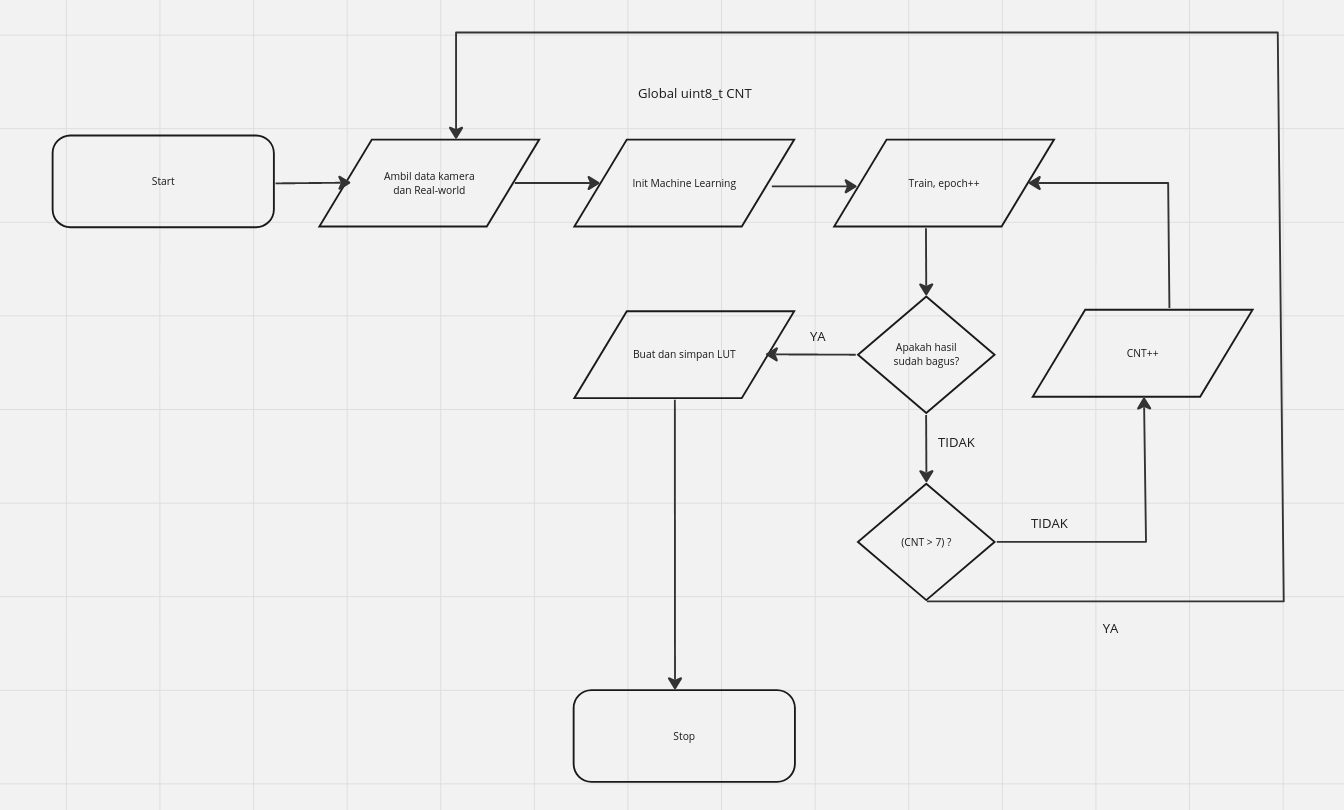
\includegraphics[width=0.4\textwidth]{gambar/desain_sistem.png}

  % Ubah sesuai dengan keterangan gambar yang diinginkan.
  \caption{Desain Sistem Kalibrasi.}
  \label{fig:desainsistem}
\end{figure}

Pada desain sistem yang digunakan, terdapat beberapa tahapan proses yang dilakukan. Tahapan tersebut adalah sebagai berikut:

\begin{enumerate}
  \item \textbf{Pengambilan Data}: Pada tahapan ini, data yang diambil adalah data koordinat titik pada kamera dan data koordinat titik pada dunia nyata.
  \item \textbf{Machine Learning}: Pada tahapan ini, data koordinat yang telah diambil akan dilakukan proses \emph{training} menggunakan metode \emph{Machine Learning}. Adapun metode yang digunakan adalah \emph{Neural Network}.
  \item \textbf{Pembuatan \emph{Lookup Table}}: Pada tahapan ini, hasil dari \emph{training} akan digunakan untuk membuat \emph{lookup table} yang akan digunakan untuk kalibrasi kamera. \emph{Lookup table} dibuat dengan mengunakan dua \emph{byte memory} untuk setiap koordinat titik pada kamera.
\end{enumerate}

\subsection{Implementasi pada Robot}
\label{subsec:implementasi}

Implementasi dari sistem kalibrasi kamera omnivision menggunakan \emph{Machine Learning} dilakukan melalui beberapa tahapan. Tahapan tersebut adalah sebagai berikut: 

\begin{enumerate}
  \item \textbf{\emph{Load Lookup Table}}: Pada tahapan ini, \emph{lookup table} yang telah dibuat akan dimuat ke dalam program dalam bentuk \emph{array}. 
  \item \textbf{Kalibrasi Kamera}: Pada tahapan ini, kamera akan diarahkan ke titik yang telah ditentukan. Kemudian, kamera akan mengambil gambar dan mengirimkan data koordinat titik ke program. Program akan mengubah data koordinat tersebut menjadi data koordinat yang benar berdasarkan \emph{lookup table}.
\end{enumerate}